\documentclass{article}
\usepackage[utf8]{inputenc}
\usepackage[margin=1.2in]{geometry}
\usepackage{hyperref}

\usepackage{tikz}
\usetikzlibrary{positioning}

\usepackage{natbib}
\usepackage{graphicx}
\usepackage{amsmath}
\usepackage{listings}
\usepackage{xcolor}


\definecolor{codegreen}{rgb}{0,0.6,0}
\definecolor{codegray}{rgb}{0.5,0.5,0.5}
\definecolor{codepurple}{rgb}{0.58,0,0.82}
\definecolor{backcolour}{rgb}{0.95,0.95,0.92}
\definecolor{deepblue}{rgb}{0,0,0.5}
\definecolor{deepred}{rgb}{0.6,0,0}
\definecolor{deepgreen}{rgb}{0,0.5,0}

\lstdefinestyle{mystyle}{
    backgroundcolor=\color{white},   
    commentstyle=\color{codegreen},
    keywordstyle=\color{deepblue},
    numberstyle=\tiny\color{codegray},
    stringstyle=\color{deepgreen},
    emph={Agent,__init__,act,self,union,exists, scope},
    emphstyle=\color{deepred},
    basicstyle=\ttfamily\footnotesize,
    breakatwhitespace=false,         
    breaklines=true,                 
    captionpos=b,                    
    keepspaces=true,                 
    numbers=left,                    
    numbersep=5pt,                  
    showspaces=false,                
    showstringspaces=false,
    showtabs=false,                  
    tabsize=3
}

\lstset{style=mystyle}

\title{\vspace{-2 cm}Universidade Federal de Ouro Preto \\ BCC 325 - Inteligência Artificial \\ Problemas de Satisfação de Restrições}
\author{Prof. Rodrigo Silva}
\date{}


\begin{document}

\maketitle

\section{Material de apoio}

\begin{itemize}
    \item Capítulo 8 do Livro\textit{ Artificial Intelligence: Foundations of Computational Agents,  2nd Edition} disponível em \textit{https://artint.info/}
    \item \url{https://www.youtube.com/watch?v=aircAruvnKk&list=PLZHQObOWTQDNU6R1_67000Dx_ZCJB-3pi}
    \item \url{https://aibyhand.substack.com/t/workbook}
    \item Aquele que tudo sabe, tudo vê e nada teme.
\end{itemize}

\section{Exercícios}


\begin{enumerate}

    \item \url{https://aibyhand.substack.com/p/w3-linear-layer}
    \item \url{https://aibyhand.substack.com/p/w4-activation}
    \item \url{https://aibyhand.substack.com/p/w5-artificial-neuron}
    \item \url{https://aibyhand.substack.com/p/w6-batch}
    \item \url{https://aibyhand.substack.com/p/w7-connection}
    \item \url{https://aibyhand.substack.com/p/w8-hidden-layer}
    \item \url{https://aibyhand.substack.com/p/w9-deep}
    \item \url{https://aibyhand.substack.com/p/w10-wide}
    \item \url{https://aibyhand.substack.com/p/w11-softmax}

    \item  Considere a rede neural abaixo:
    
    \begin{figure}[!ht]
        \centering
        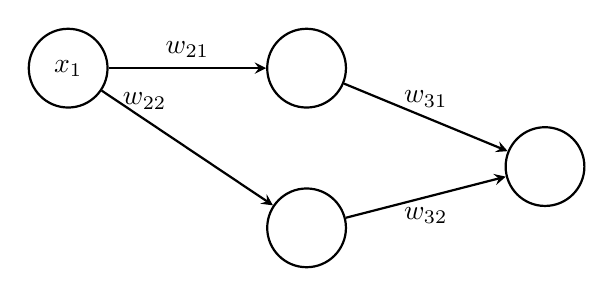
\begin{tikzpicture}[%
            neuron/.style={circle, draw, thick, minimum size=1cm},
            arrow/.style={->,>=stealth,thick}
        ]
        
        % Input neurons
        \node[neuron] (input1) at (0,0) {$x_1$};
        %\node[neuron] (input2) [below=of input1] {$x_2$};
        
        % Hidden layer neurons
        \node[neuron] (hidden1) [right=2cm of input1] {};
        \node[neuron] (hidden2) [below=of hidden1] {};
        
        % Output neuron
        \node[neuron] (output) [right=2cm of hidden1, yshift=-1.25cm] {};
        
        % Connect input layer to hidden layer
        \draw[arrow] (input1) -- (hidden1) node[midway, above] {$w_{21}$};
        \draw[arrow] (input1) -- (hidden2) node[near start, above] {$w_{22}$};
        %\draw[arrow] (input2) -- (hidden1) node[near start, below] {$w_{12}$};
        %\draw[arrow] (input2) -- (hidden2) node[midway, below] {$w_{22}$};
        
        % Connect hidden layer to output layer
        \draw[arrow] (hidden1) -- (output) node[midway, above] {$w_{31}$};
        \draw[arrow] (hidden2) -- (output) node[midway, below] {$w_{32}$};
        
        \end{tikzpicture}
    \end{figure}

    Esta rede não possui termos de viés (bias) e tem como funções de ativação a função ReLU (Rectified Linear Unit) que pode ser definida como:

    \begin{equation}
        \text{ReLU}(x) = \max(0, x)
    \end{equation}

    A derivada da ReLU é definida como:

    \begin{equation}
            \frac{d}{dx}(\text{ReLU}(x)) =
            \begin{cases}
            1 & \text{if } x > 0 \\
            0 & \text{if } x \leq 0
            \end{cases}            
    \end{equation}

    Obtenha o gradiente do erro quadrado em relação aos pesos da rede. Todos os passos da derivação da gradiente devem ser apresentados.


    \item  Considere a rede neural abaixo:
    
    \begin{figure}[!ht]
        \centering
        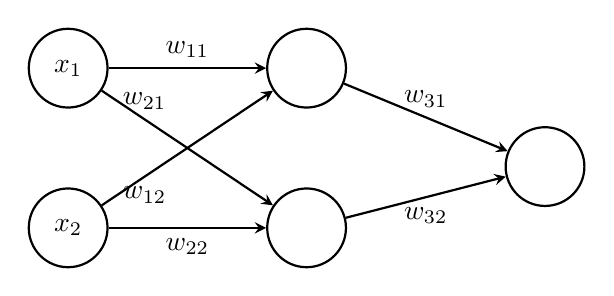
\begin{tikzpicture}[%
            neuron/.style={circle, draw, thick, minimum size=1cm},
            arrow/.style={->,>=stealth,thick}
        ]
        
        % Input neurons
        \node[neuron] (input1) at (0,0) {$x_1$};
        \node[neuron] (input2) [below=of input1] {$x_2$};
        
        % Hidden layer neurons
        \node[neuron] (hidden1) [right=2cm of input1] {};
        \node[neuron] (hidden2) [right=2cm of input2] {};
        
        % Output neuron
        \node[neuron] (output) [right=2cm of hidden1, yshift=-1.25cm] {};
        
        % Connect input layer to hidden layer
        \draw[arrow] (input1) -- (hidden1) node[midway, above] {$w_{11}$};
        \draw[arrow] (input1) -- (hidden2) node[near start, above] {$w_{21}$};
        \draw[arrow] (input2) -- (hidden1) node[near start, below] {$w_{12}$};
        \draw[arrow] (input2) -- (hidden2) node[midway, below] {$w_{22}$};
        
        % Connect hidden layer to output layer
        \draw[arrow] (hidden1) -- (output) node[midway, above] {$w_{31}$};
        \draw[arrow] (hidden2) -- (output) node[midway, below] {$w_{32}$};
        
        \end{tikzpicture}
    \end{figure}

    $w_{11}$ = $w_{21}$ = $w_{12}$ = $w_{22}$ = $w_{31}$ = $w_{32}$ = 1

    Esta rede tem como funções de ativação a função ReLU (Rectified Linear Unit) que pode ser definida como:

    \begin{equation}
        \text{ReLU}(x) = \max(0, x)
    \end{equation}

    A derivada da ReLU é definida como:

    \begin{equation}
            \frac{d}{dx}(\text{ReLU}(x)) =
            \begin{cases}
            1 & \text{if } x > 0 \\
            0 & \text{if } x \leq 0
            \end{cases}            
    \end{equation}


    \begin{enumerate}
        \item Calcule o gradiente do erro quadrado em relação à $w_{32}$ quando $\mathbf{x} = [2,1]$ e $y = 20$.
        \item Calcule o gradiente do erro quadrado em relação à $w_{22}$ quando $\mathbf{x} = [2,1]$ e $y = 20$. 
        \item Como $w_{32}$ e $w_{22}$ devem ser alterados de forma a diminuir o erro?   
    \end{enumerate}
    


\end{enumerate}


\end{document}

